\documentclass[12pt,a4paper]{article}
\usepackage[utf8]{inputenc}
\usepackage[italian]{babel}
\usepackage[dvipsnames]{xcolor}
\usepackage{amsthm}
\usepackage{amsmath}
\usepackage{mathtools}
\usepackage{booktabs}
\usepackage{tabularx}
\usepackage{multicol}
\usepackage{multirow}
\usepackage{graphicx}
\usepackage{fixltx2e}
\usepackage{mathrsfs}
\usepackage{amsfonts}
\usepackage{makeidx}
\usepackage[hidelinks]{hyperref}
\usepackage{relsize}
\usepackage{array}
\usepackage{minted}
\usepackage{fullpage}
\usepackage{dsfont}
\usepackage{amssymb}
\usepackage[final]{pdfpages}
\usepackage{eurosym}
\usepackage{tabto}
\usepackage{pifont}
\usepackage{tikz}
\usepackage{verbatim}
\usepackage{attachfile}
\usepackage{color}
\usepackage{comment}
\usetikzlibrary{arrows.meta}
\usepackage{vwcol}  
\usepackage{lipsum}
\usepackage{microtype}
\usepackage{cleveref}
\usepackage{frcursive}
\usepackage[T1]{fontenc}
\usepackage{bbding}
\usepackage{pifont}
\usetikzlibrary{shapes.multipart}
\usetikzlibrary{arrows,positioning,automata,backgrounds,shapes}
\usepackage[dvipsnames]{xcolor}

\usepackage{fancyvrb}

% redefine \VerbatimInput
\RecustomVerbatimCommand{\VerbatimInput}{VerbatimInput}%
{fontsize=\footnotesize,
 %
 frame=lines,  % top and bottom rule only
 framesep=2em, % separation between frame and text
 rulecolor=\color{Gray},
 %
 label=\fbox{\color{Black}data.txt},
 labelposition=topline,
 %
 commandchars=\|\(\), % escape character and argument delimiters for
                      % commands within the verbatim
 commentchar=*        % comment character
}
\newcommand\finline[3][]{\begin{myfont}[#1]{#2}#3\end{myfont}}%
\addto\captionsitalian{\renewcommand{\appendixname}{Allegato}}
\newcommand{\xmark}{\ding{55}}%


\hypersetup{
  pdfborder = {0 0 0}
}

\newtheoremstyle{thm}% name of the style to be used
  {3pt}% measure of space to leave above the theorem. E.g.: 3pt
  {3pt}% measure of space to leave below the theorem. E.g.: 3pt
  {\itshape}% name of font to use in the body of the theorem
  {0pt}% measure of space to indent
  {\bfseries}% name of head font
  {}% punctuation between head and body
  { }% space after theorem head; " " = normal interword space
  {\thmname{#1}\thmnumber{ #2} \thmnote{\bf (#3)}\\}% Manually specify head
  
\newtheoremstyle{def}% name of the style to be used
  {3pt}% measure of space to leave above the theorem. E.g.: 3pt
  {3pt}% measure of space to leave below the theorem. E.g.: 3pt
  {\normalfont}% name of font to use in the body of the theorem
  {0pt}% measure of space to indent
  {\bfseries}% name of head font
  {}% punctuation between head and body
  { }% space after theorem head; " " = normal interword space
  {\thmname{#1}\thmnumber{ #2} \thmnote{\bf (#3)}\\}% Manually specify head
  
%\newcommand\stareq{\stackrel{\mathclap{\normalfont\mbox{*}}}{=}}

\theoremstyle{thm}
\newtheorem{theorem}{Teorema}[section]
\newtheorem{lemma}[theorem]{Lemma}
\newtheorem{proposition}[theorem]{Proposizione}
\newtheorem{corollary}[theorem]{Corollario}
\theoremstyle{def}
\newtheorem{definition}{Definizione}[section]

\tikzset{
    mynode/.style={rectangle,rounded corners,draw=black, top color=white, bottom color=yellow!50,very thick, text centered},
    myarrow/.style={->, >=latex', shorten >=1pt, thick},
    mylabel/.style={text width=7em, text centered} 
}


\begin{document}

\begin{titlepage}
\begin{center}
\vspace{3cm}

\begin{center}

\includegraphics[scale=0.3]{Cherubino.jpg}
\end{center}

\vspace{1cm}
\Huge
{\sc Singular Value Decomposition}\\
for\\
{\sc Latent Semantic Index}\\
in\\
{\sc Recommendation Systems}\\
\Large
Anno Accademico 2016/2017\\

\vspace{1.5cm}

\Large
A cura di\\
{\sc Gemma Martini}\\

\vspace{1.5cm}

\today

\vfill

\end{center}
\end{titlepage}

%%%%%%%%%%%%%%%%%%%~~~~~~~~~~~~~~~~~~~~~~~~~~~~~~~~~~~~~~~~~~~%%%%%%%%%%%%%%%%%%%%%

\tableofcontents
\newpage

%TODO: rivedere definizione di B e C
%TODO: 
%TODO: 
%%%%%%%%%%%%%%%%%%%~~~~~~~~~~~~~~~~~~~~~~~~~~~~~~~~~~~~~~~~~~~%%%%%%%%%%%%%%%%%%%%%
							
\section{Introduzione}
L'insegnamento è da secoli guidato dalla figura di un docente, che propone ad un gruppo (talvolta composto da un solo elemento) di studenti un insieme di tematiche, secondo un ordinamento che possa facilitarne l'apprendimento.

L'obiettivo di questa trattazione è di valutare l'utilità della \textit{singular value decomposition} (da qui SVD) e del {\it latent semantic indexing} (in seguito LSI) applicati ai \textit{recommendation system} per la piattaforma di allenamento per le Olimpiadi Italiane di Informatica, il \textit{Contest Management System} (da qui CMS), con l'obiettivo di suggerire agli utenti iscritti quali argomenti (o meglio problemi) affrontare.

Si assume nel lettore la conoscenza della SVD, ma è possibile trovare, per i meno esperti, le nozioni teoriche necessarie per spiegare LSI, in appendice \ref{appendice1}.


%%%%%%%%%%%%%%%%%%%~~~~~~~~~~~~~~~~~~~~~~~~~~~~~~~~~~~~~~~~~~~%%%%%%%%%%%%%%%%%%%%%
							
\section{La teoria}

                      %~~~~~~~~~~~~~~~~~~~~~~~~~~~~~~~%

\subsection{Latent Semantic Indexing}
L'obiettivo teorico di questo algoritmo è la modellazione dei dati su un sistema, in modo da ottenere informazioni concise, ma espressive circa le grandezze in gioco.

Più in dettaglio, nella prima parte vengono gettate le fondamenta per introdurre lo \textit{sketch}, che rappresenta sinteticamente le informazioni sugli utenti e sui \textit{task}. Nella seconda parte, in base a questo \textit{sketch}, viene definita la \textbf{somiglianza} di più utenti tra loro.

                                %~~~~~~~~~%

\subsubsection{I dati}
\label{dati}
\begin{description}
\item[{\sc Sia}] $T$ un insieme di problemi di cardinalità $t$.
\item[{\sc Sia}] $P$ l'insieme degli utenti che hanno accesso alla piattaforma (e quindi ai $t$ \textit{task}), con $|P| = p$.
\item[{\sc Sia}] $M \in M(p,t,\mathds{N})$ la matrice dei punteggi totalizzati dagli utenti di $P$ sui \textit{task} di $T$. In particolare $(m_{ij})$ è uguale al punteggio ottenuto da $p_i$ sul \textit{task} $t_j$.
\item[{\sc Sia}] $B=M^tM \in S(t, \mathds{N})$ la matrice di elementi $(b_{ij})$, che rappresentano la somiglianza tra i due \textit{task} $t_i$ e $t_j$.
\item[{\sc Sia}] $C=MM^t \in S(p, \mathds{N})$ la matrice di elementi $(c_{i,j})$, che rappresentano la somiglianza tra l'utente $p_i$ e l'utente $p_j$.
\end{description}

                                %~~~~~~~~~%

\subsubsection{Il modello}
\label{k}
Con i dati definiti come sopra è possibile decomporre $M$ mediante SVD, ottendendo tre matrici:
\begin{description}
\item[{\sc Matrice sinistra dei vettori singolari}] $S \in M(p,r,\mathds{R})$
\item[{\sc Matrice destra dei vettori singolari}] $U \in M(t,r,\mathds{R})$
\item[{\sc Matrice diagonale dei valori singolari}] $\Sigma \in D(r,\mathds{R})$
\end{description}
tali che $M=S\Sigma U^t$.
La matrice $\Sigma$ ha, sulla diagonale, elementi decrescenti; di conseguenza gli ultimi elementi possono essere trascurati.
Si può decidere di ridurre la matrice $\Sigma$ ad una matrice in $M(k, \mathds{R})$, ottenendo $\Sigma_k$, $S_k$ e $U_k$, per calcoli più veloci e per ridurre il rumore dovuto a dati non significativi.

$M_k = S_k \Sigma_k U_k^t$ è di dimensione $p \times t$, come $M$, e la approssima.

                                %~~~~~~~~~%

\subsubsection{Informazioni nascoste}
\label{sym}
In modo un po' informale è possibile definire che cos'è un' ``informazione nascosta'': come la diagonalizzazione di una matrice descrive, tramite gli autovettori, delle direzioni privilegiate dalle quali guardare la trasformazione, così gli autovettori in $S$ ed in $U$ rappresentano l'informazione sui problemi e  sugli utenti in modo più comodo.

Lo \textit{sketch} di questo algoritmo risiede nell'interpretazione di $S_k \Sigma_ k$ e $\Sigma_k U_k^t$ come rappresentazione essenziale rispettivamente di utenti e \textit{task} in termini di combinazione delle informazioni nascoste.

Concludendo, la \textbf{somiglianza} tra più utenti è espressa dalla distanza del coseno tra i due vettori $p_i$ e $p_j$, ossia $\frac{p_i p_j}{|p_i||p_j|}$.

                                 %~~~~~~~~~%

\subsubsection{Vicini}
\label{ilCento}
Una volta trovato un modo efficace di individuare la somiglianza tra utenti, è necessario selezionare, per ogni utente $p_i$ un certo numero $h$ di utenti ``simili'', individuati dall'insieme $Closest(p_i)$. Questo espediente è fondamentale per collezionare informazioni utili sulle capacità di soluzione degli utenti ``simili'', così da poter individuare una lista di suggerimenti per l'utente preso in esame.

Un modo per quantificare la fattibilità di un \textit{task} nella cerchia dei vicini dell'utente $p_i$ è quello di ottenere la frequenza di soluzione di ogni \textit{task} su quegli utenti, in termini più formali

~~~~~~~~~~~~~~~~~~~~~~$\forall t_j :$ $m_{i,j} \neq 100$ $freq(t_j) = \sum\limits_{\substack{p_s \in Closest(p_i) \\ m_{s,j} = 100}} m_{s,j}$ 

In base a questo calcolo si ottiene un ordinamento sui \textit{task} non risolti dall'utente $p_i$, che riflette la loro propedeuticità per quell'utente.

%%%%%%%%%%%%%%%%%%%~~~~~~~~~~~~~~~~~~~~~~~~~~~~~~~~~~~~~~~~~~~%%%%%%%%%%%%%%%%%%%%%
\section{La pratica}

                      %~~~~~~~~~~~~~~~~~~~~~~~~~~~~~~~%

\subsection{La piattaforma}
Il sito di allenamenti \url{https://cms.di.unipi.it/#/overview} offre qualche centinaia di problemi o \textit{task} agli utenti iscritti, da risolvere senza limiti di tempo nè di numero di sottomissioni. Ad ogni sottomissione viene assegnato un punteggio che va da $0$ a $100$. Il sistema tiene come \textit{score} su quel problema il migliore tra i punteggi ottenuti su quel determinato \textit{task} da quell'utente.

                      %~~~~~~~~~~~~~~~~~~~~~~~~~~~~~~~%

\subsection{Le assunzioni}
Nella fusione fra teoria e pratica è necessario definire dettagliatamente il sistema in oggetto e precisare tutte le assunzioni, come segue:
\begin{description}
\item[{\sc Selezione dei dati}] I dati sul sistema sono talvolta fuorvianti, nel senso che esistono \textit{task} sui quali nessun utente si è cimentato ed esistono utenti che nonhanno provato a risolvere nemmeno un \textit{task}. Per eliminare errori dovuti a questa situazione si è deciso di non tener traccia di tali valori nella costruzione della matrice.
\item[{\sc Suggerimenti propedeutici}] Nella sezione \ref{ilCento} si prendono in considerazione come \textit{task} suggeriti quelli sui quali l'utente in considerazione non ha totalizzato punteggio pieno ($100$ punti) su quel problema. La scelta è stata fatta considerando che potrebbe essere formativo riuscire a risolvere completamente un certo \textit{task} prima di passare al successivo, poichè aggiungere anche solo pochi punti allo \textit{score} potrebbe risultare decisivo nel processo di apprendimento.
\item[{\sc Sparsità della matrice}] Dalle evidenze sperimentali e dai risultati ottenuti da \textit{Badrul M. Sarwar} et al.\footnote{Application of Dimensionality Reduction in Recommender System -- A Case Study by Badrul M. Sarwar, George Karypis, Joseph A. Konstan, John T. Riedl} si è deciso di utilizzare la matrice $(user, task)$ desparsificata, dove sono sostiuiti ai valori $0$ la media dei punteggi di tutti gli utenti su quel \textit{task}.
\end{description}

                      %~~~~~~~~~~~~~~~~~~~~~~~~~~~~~~~%

\subsection{La scelta dei parametri}
Prima ancora di arrivare al codice vero e proprio è necessario fare alcune considerazioni sulla \textbf{scelta dei parametri}. Nella sezione \ref{k} si parla di $k$, indice con il quale ridurre la taglia delle matrici che decompongono $M$, per abbassare rumore e complessità di calcolo. Inoltre, nella sezione \ref{ilCento} viene introdotto il valore $h$, che indica il numero di vicini più simili rispetto ad un certo utente $i$ da considerare per trovare i suggerimenti.

La scelta di tali parametri deve essere valutata, infatti intuitivamente la matrice $M_k$ può essere confrontata con $M$ per differenza. Applicando la norma di Frobenius alla differenza tra le due matrici si nota che essa tende a $0$ col crescere di $k$. Quindi il metodo di scelta di $k$ non può basarsi sul valore di tale norma, perchè il risultato è chiaramente il $k$ massimo.

Per individuare i valori di $k$ e $h$ con i quali si ottengono suggerimenti più verosimili è stato scelto di confrontare uno \textit{screenshot} di CMS di un mese fa ed uno di adesso, valutando \textit{precision} e \textit{recall} dei risultati prodotti dall'algoritmo. In particolare, sia $A = (a_{i, j}) = \biggl\lfloor \frac{M_{fine}}{100} \biggr\rfloor - \biggl\lfloor \frac{M_{inizio}}{100} \biggr\rfloor$, la \textbf{bontà} dell'algoritmo sui vari parametri è stata calcolata come segue:
\[
goodness(k, h) = \sum\limits_{p_i \in P}  g(p_i)
\]
con
\[
g(p_i) = \Biggl\{
		\begin{array}{ll}
			- l, ~~~~~~~~~~~~~~~se ~ A_{i, j} = 1 ~ e ~ t_j \not\in s_i\\
			l + 1 - pos(t_j), ~ ~ se ~ A_{i, j} = 1 ~ e ~ t_j \in s_i\\
		\end{array}
\]
dove $s_i$ è il vettore dei \textit{task} suggeriti all'utente $i$ e $pos(t_j)$ è la posizione del \textit{task} $j$ all'interno di $s_i$.

%%%%%%%%%%%%%%%%%%%~~~~~~~~~~~~~~~~~~~~~~~~~~~~~~~~~~~~~~~~~~~%%%%%%%%%%%%%%%%%%%%%
\section{Implementazione}

                      %~~~~~~~~~~~~~~~~~~~~~~~~~~~~~~~%

\subsection{La struttura}
L'algoritmo descritto sopra è stato implementato in \textit{Python}, perchè potesse essere facilmente inserito sulla piattaforma.

Si struttura in due soli file:
\begin{description}
\item[{\tt algorithm.py}] Contiene solo lo scheletro dell'algoritmo, con un minimo di UI ed una struttura dati \texttt{Useful}, istanziata con \texttt{myData}, in modo da incapsulare gli elementi importanti
\item[{\tt functions.py}] È il vero e proprio pilastro del programma: definisce le funzioni usate da \texttt{algorithm.py} ed alcune funzioni ausiliare, per rendere il codice più snello. Di seguito una breve descrizione di funzioni e procedure principali:
	\begin{itemize}
	\item \texttt{deSparsify} modifica la struttura dati rendendo la matrice non sparsa. Si noti che questa funzione può essere chiamata oppure no, a seconda della scelta dell'utente. La funzione calcola, per ogni \textit{task} $j$, la media dei punteggi totalizzati dagli utenti su quel \textit{task} e sostiuisce gli $0$ sulla colonna $M^j$ con il valore calcolato.
	\item \texttt{tasksAndPeopleCountAndHash} inizializza alcuni campi della struttura dati e stabilisce una funzione di \textit{hash} per ottenere una matrice più ``sintetica'' possibile. Infatti, del file di testo che rappresenta CMS in un dato istante, non è che fuorviante prendere in considerazione gli utenti iscritti che non hanno mai inviato una sottomissione o i problemi che non sono mai stati provati da nessun partecipante. 
	\item \texttt{parseMatrix} si occupa di leggere e memorizzare i valori dal file nella matrice e di chiamare \texttt{tasksAndPeopleCountAndHash}.
	\item \texttt{reduceToSVDk} chiama le funzioni sopracitate aggiornando la struttura dati \texttt{myData}, dopodichè riduce $M$ tramite SVD e riduce in base a $k$ le dimensioni delle matrici $S$ e $\Sigma$.
	\item \texttt{userConceptProduct} modifica la struttura dati inizializzando e aggiornando gli elementi della matrice che ha in posizione $(i, j)$ la somiglianza tra l'utente $i$ e l'utente $j$, come definita alla sezione \ref{sym}.
	\item \texttt{recommendationsl} per ogni utente restituisce il vettore degli utenti a lui ``simili'' in ordine decrescente si somiglianza.
	\item \texttt{printMatrix} si occupa di scrivere a video in modo ordinato i risultati ottenuti.
	\end{itemize}
\end{description}

Si verifica facilmente che l'operazione con costo computazionale maggiore è il calcolo dell'SVD.

Di seguito un diagramma che indica la relazione d'uso tra le varie funzioni/procedure:

\begin{center}
\vspace{2cm}
  \begin{tikzpicture}[>=stealth',node distance=3cm,on grid,initial/.style ={}]
    \node[mynode] (11) [] {main di {\tt algorithm.py}};
    \node[mynode] (21) [below  left =of 11] {\tt reduceToSVDk};
    \node[mynode] (22) [below  =of 11] {\tt userConceptProduct};
    \node[mynode] (23) [below  right=of 11] {\tt recommendationsl};
    \node (20) [left =4cm of 21, minimum height=0.6cm] {};
    \node[mynode] (31) [below left =of 21] {\tt parseMatrix};
    \node[mynode] (32) [below =of 21] {\tt deSparsify};
    \node[mynode] (33) [below =of 22] {\tt userConceptNormalized};
    \node[mynode] (34) [below right =of 23] {\tt tasksFrequency};
    \node (30) [below =3cm of 31] {};
    \node[mynode] (41) [below =of 31] {\tt TasksAndPeopleCountAndHash};
    \node[mynode] (42) [below right =of 34] {\tt closesth};
    \node[mynode] (43) [below =of 34] {\tt taskFrequency};
    \node[mynode] (51) [below right =of 42] {\tt neighboursi};
    \path (11) edge [myarrow]   node {} (21)
          (11) edge [myarrow]   node {} (22)
          (11) edge [myarrow]   node {} (23)
          (21) edge [myarrow]   node {} (31)
          (21) edge [myarrow]   node {} (32)
          (22) edge [myarrow]   node {} (33)
          (23) edge [myarrow]   node {} (34)
          (31) edge [myarrow]   node {} (41)
          (34) edge [myarrow]   node {} (42)
          (34) edge [myarrow]   node {} (43)
          (42) edge [myarrow]   node {} (51);

  \end{tikzpicture}
\end{center}

Per quanto riguarda la scelta dei parametri $k$ e $h$, il codice è stato scritto in \textit{Bash} (per iterare su tutte le coppie e per ridirigere input ed output) ed in \textit{Python} (per eseguire i veri e propri conti, avvalendosi di strutture dati per migliorare il costo computazionale).

Il codice integrale per effettuare tali prove si trova in appendice \ref{appendice2}, fatta eccezione per le funzioni ausiliarie, che sono le stesse del codice che segue.
                      %~~~~~~~~~~~~~~~~~~~~~~~~~~~~~~~%

\subsection{Il codice}

                                %~~~~~~~~~%

\subsubsection{\tt algorithm.py}
\begin{minted}[mathescape,
               linenos,
               numbersep=5pt,
               frame=lines,
               framesep=2mm]{python}
import math
import random
import sys
import numpy as np
import readline
from numpy import linalg as LA
from functions import *

"""Struttura dati necessaria per lo storage compattato delle
	informazioni"""
class Useful:
	def __init__(self, k, h, l):
		self.k = k
		self.h = h
		self.l = l	

k = 28 #Miglior valore dai test
h = 61 #Numero di vicini da considerare, miglior valore dai test
l = 20 #Numero di suggerimenti, a scelta

print('Recommendation system for CMS')
inputFile  = open("punteggi.txt", "r")
var = input('Press y for recommendations from desparsified matrix, \
press n for recommendations from the original one -> ')
myData = Useful(k, h, l)
if(var == 'y'):
	reduceToSVDk(inputFile, myData, 'yes')
else:			
	reduceToSVDk(inputFile, myData, 'no')
suggestionsMatrix = np.empty([myData.p,myData.l], dtype = int)
userConceptProduct(myData)
for useri in range(0, myData.p):
	indexesTasks = recommendationsl(useri, myData)
	for task in range(0, myData.l):
		suggestionsMatrix[useri, task] = indexesTasks[task]
#Comunicazione risultati
var = input('Press a for all the results, press u for a specific user s \
suggestions -> ')
#Nota: solo nell'operazione di print sono applicate le funzioni inverse 
#delle funzioni di hash
if(var == 'a'):
	printMatrix(suggestionsMatrix, myData)
else:
	user = input('Insert the user number -> ')
	printRow(suggestionsMatrix, user, myData)

               
\end{minted}

                                %~~~~~~~~~%

\subsubsection{\tt functions.py}
\begin{minted}[mathescape,
               linenos,
               numbersep=5pt,
               frame=lines,
               framesep=2mm]{python}
import math
import random
import sys
import numpy as np
from numpy import linalg as LA


"""Questa funzione prende l'oggetto myData e aggiorna:
	(1) M -> rendendola non sparsa"""
def deSparsify(myData):
	#ciclo sulle colonne (task)
	for task in range(0, myData.t):
		average = 0
		for counter in range(0, myData.p):
			average = average + myData.M[counter, task]
		average = average/myData.p
		for counter in range(0, myData.p):
			if (myData.M[counter, task] == 0):
				 myData.M[counter, task] = average

"""Questa funzione prende il file di input e l'oggetto myData e
	inizializza:
	(1) t -> numero di task
	(2) p -> numero di utenti
	(3) hashPeople -> lista di interi che rappresentano gli utenti
	(4) hashTasks -> lista di interi che rappresentano i task"""
def tasksAndPeopleCountAndHash(inputFile, myData):
	tasksSet = set()
	peopleSet = set()
	data = inputFile.readlines()
	lines = []
	for line in data:
		words = list(map(int, line.split()))
		tasksSet.add(words[1])
		peopleSet.add(words[0])
		lines.append(words)
		
	myData.t = len(tasksSet)
	myData.p = len(peopleSet)
	myData.hashPeople = sorted(list(peopleSet))
	myData.hashTasks = sorted(list(tasksSet))
	return lines

"""Questa funzione prende il file di input e l'oggetto myData e
	inizializza:
	(1) M -> matrice che ha come righe gli utenti e per colonne i task
	(2) t, p, hashPeople, hashTasks -> con tasksAndPeopleCountAndHash"""
def parseMatrix(inputFile, myData):
	lines = tasksAndPeopleCountAndHash(inputFile, myData)
	myData.M = np.zeros((myData.p,myData.t)) 
	for words in lines:
		myData.M[myData.hashPeople.index(words[0]),
		myData.hashTasks.index(words[1])] = words[2]

"""Questa funzione prende il file di input, l'oggetto myData ed un flag ed
	inizializza:
	(1) Sigmak -> matrice risultante da SVD, ma ridotta in taglia
	(2) Sk -> matrice risultante da SVD, ma ridotta in taglia
	(3) M, t, p, hashPeople, hashTasks -> mediante parseMatrix
	(4) aggiorna M (forse) -> mediante deSparsify"""
def reduceToSVDk(inputFile, myData, flag):
	#Parsa il file in una matrice
	parseMatrix(inputFile, myData)
	#Valuta il flag
	if (flag == 'yes'):
		deSparsify(myData)
	#Calcola la SVD di M
	S, Sigma, U = np.linalg.svd(myData.M, full_matrices=False)
	#Approssima M
	myData.Sigmak = np.diag(Sigma[0:myData.k])
	myData.Sk = S[...,0:myData.k]

"""Questa funzione prende l'utente user e l'oggetto myData e restituisce:
	(1) Il vettore di dimensione k, che rappresenta il concetto di
		quell'utente"""
def userConceptNormalized(user, myData):
	rowOfSk = myData.Sk[user]
	userCon = np.matmul(rowOfSk, myData.Sigmak)
	norm = LA.norm(userCon)
	userConNorm = userCon/norm
	return userConNorm

"""Questa funzione prende l'oggetto myData ed inizializza:
	(1) MatRes -> matrice della somiglianza tra utenti"""
def userConceptProduct(myData):
	Un = np.empty([myData.p, myData.k], dtype = float)
	for user in range(0, myData.p):
		Un[user] = userConceptNormalized(user, myData)
	myData.MatRes = np.matmul(Un, Un.transpose())
	
"""Questa funzione prende un utente useri e l'oggetto myData e ritorna:
	(1) neighboursi -> vettore delle somiglianze tra useri e gli
		altri utenti"""
def neighboursUi(useri, myData):
	neighboursi = np.empty([myData.p], dtype = float)
	neighboursi = myData.MatRes[useri]
	#A neigbours[useri] è assegnato un valore che non disturba
	#la somiglianza
	neighboursi[useri] = 0
	return neighboursi

"""Questa funzione prende un utente useri e l'oggetto myData e ritorna:
	(1) indexes -> vettore degli interi che rappresentano gli h
		utenti più simili a useri, ordinati in senso decrescente"""
def closesth(useri, myData):
	indexes = np.empty([myData.h], dtype = int)
	neighboursi = neighboursUi(useri, myData)
	minimum = min(neighboursi)
	for counter in range(0, myData.h):
		indexes[counter] = np.argmax(neighboursi)
		neighboursi[np.argmax(neighboursi)] = minimum -1
	return indexes

"""Questa funzione prende l'oggetto myData, un task e indexes e
	restituisce:
	(1) frequency -> frequenza di un task su tutti gli h utenti
		di indexes"""
def taskFrequency(myData, task, indexes):
	frequency = 0
	for counter in range(0, myData.h):
		frequency = frequency + myData.M[indexes[counter], task]
	return frequency

"""Questa funzione prende un utente useri e l'oggetto myData e ritorna:
	(1) frequencies -> array delle frequenze di ogni task per
		quell'utente"""
def tasksFrequency(useri, myData):
	frequencies = np.empty([myData.t], dtype = int)
	indexes = closesth(useri, myData)
	for task in range(0, myData.t): 
		frequencies[task] = taskFrequency(myData, task, indexes)
	return frequencies

"""Questa funzione prende un utente useri e l'oggetto myData e
	restituisce:
	(1) indexesTasks -> vettore dei primi l suggerimenti
		(tra i task non risolti completamente) per l'utente useri"""
def recommendationsl(useri, myData):
	indexesTasks = np.empty([myData.l], dtype = int)
	frequencies = tasksFrequency(useri, myData)
	minimum = min(frequencies)
	counter = 0
	while counter < myData.l:
		currentTask = np.argmax(frequencies)
		frequencies[currentTask] = minimum -1
		if (myData.M[useri, currentTask] != 100):
			indexesTasks[counter] = currentTask
			counter = counter + 1
	return indexesTasks

"""Questa funzione prende la matrice suggestionsMat e l'oggetto myData
	e chiama printRow per ogni riga, NOTA: deve passare per la
	funzione di hash"""
def printMatrix(suggestionsMat, myData):
	for user in range(0, myData.p):
		printRow(suggestionsMat, myData.hashPeople[user], myData)

"""Questa funzione prende la matrice suggestionsMat, un utente
	e l'oggetto myData e stampa a video i suggerimenti per
	quell'utente applicando la funzione la funzione inversa
	della funzione di hash sull'utente e sul task"""
def printRow(suggestionsMat, user, myData):
	print(user, end=' ')
	hashedUser = myData.hashPeople.index(int(user))
	for counter in range(0, myData.l):
		print(
		myData.hashTasks[suggestionsMat[hashedUser, counter]],
		end=' ')
	print('')		
	

\end{minted}


%%%%%%%%%%%%%%%%%%%~~~~~~~~~~~~~~~~~~~~~~~~~~~~~~~~~~~~~~~~~~~%%%%%%%%%%%%%%%%%%%%%
\section{Risultati}
Dopo aver provato tutte le coppie $(k, h)$, per valori interi di $k \in [0, \cdots, 30]$ e $h \in [0, \cdots, 300]$ è stata individuata la coppia $(28,61)$, come migliore e da qui si è svolto il vero e proprio \textit{testing} del programma. I risultati di questa parte sono discussi in maniera più dettagliata in appendice \ref{appendice2}.

Per valutare l'affidabilità dell'algoritmo ai fini di guidare l'apprendimento degli studenti si è ritenuto un valido approccio quello di richiedere proprio a loro un \textit{feedback} del prodotto.

Sono stati selezionati $5$ utenti di CMS, di età compresa tra i $16$ ed i $19$ anni, che si sono proposti di affrontare un \textit{task} per una durata di tre giorni. Il loro obiettivo è stato quello di confrontarsi col problema non tanto con lo scopo di risolverlo, quanto con lo scopo di ``valutarlo''. Si è trovato, infatti, più interessante conoscere (oltre al punteggio totalizzato) le impressioni sul problema.

Di seguito i risultati:
\begin{description}
\item[{\sc Ragazzo - 19 anni}] ha risolto il \textit{task} assegnatogli molto velocemente. L'ha ritenuto inferiore alle sue capacità (e quindi inutile nel processo di apprendimento), ma ottimo come ripasso, poichè ``era una vita che non mi allenavo su un problema greedy!''. Si è prestato per un secondo tentativo, che è risultato molto più felice, in particolare ha impiegato più tempo per risolverlo, la ricerca della soluzione lo ha coinvolto intellettualmente e ``allo stesso tempo non era esageratamente difficile, quindi direi che è stato azzeccato in pieno''.
\item[{\sc Ragazzo - 16 anni}] ha risolto il primo suggerimento in poco tempo, ma lo ha gradito molto, in quanto aveva già guardato il testo in passato e aveva iniziato a pensarci, senza però lasciare traccia di tale movimento nel sistema. Il secondo suggerimento, ricalcolato dopo la soluzione del primo, ha avuto un esito meno roseo, infatti è stato recensito come ``decisamente troppo facile''.
\item[{\sc Ragazzo - 19 anni}] ha risolto il \textit{task} assegnatogli in un tempo medio. Ritiene che il problema sia stato un buon suggerimento ``in quanto non era scontato''.
\item[{\sc Ragazzo - 19 anni}] ha risolto il problema in un tempo breve e lo ha ritenuto inferiore alle sue capacità, ma afferma che il suo profilo su CMS non corrisponde alle sue reali capacità di solutore, poichè tende a confrontarsi con problemi troppo facili.
\item[{\sc Ragazzo - 18 anni}] ha risolto il secondo problema assegnato con punteggio pieno, ha invece completamente ignorato il primo, per motivi imprecisati, cimentandosi su altri problemi. Non ha espresso alcun parere in merito, quindi non è possibile estrapolare ulteriori informazioni.
\end{description}

È ora necessario commentare un minimo questi risultati: la piattaforma CMS al momento attuale è popolata da un numero notevole di problemi di media difficoltà, quindi anche i solutori bravi possono essere vittima di una ``fluttuazione statistica'' e vedersi assegnato un \textit{task} al di sotto delle loro capacità.

Inoltre, è stato possibile verificare che in alcuni casi le capacità del solutore non sono in accordo con la difficoltà dei \textit{task} con i quali si cimenta. Come detto da alcuni dei \textit{tester}, infatti, non necessariamente i problemi che una persona svolge su CMS sono di difficoltà adeguata alle proprie capacità di soluzione. Dato che l'algoritmo ottiene informazioni solo dalla piattaforma, è naturalmente impossibile richiedere un comportamente migliore.





%%%%%%%%%%%%%%%%%%%~~~~~~~~~~~~~~~~~~~~~~~~~~~~~~~~~~~~~~~~~~~%%%%%%%%%%%%%%%%%%%%%
\section{Conclusioni}
Alla luce dei dati raccolti dalla sperimentazione si può affermare che l'algoritmo è corretto e che potrebbe rappresentare un notevole miglioramento nell'ambito di quello che è di fatto un apprendimento di tipo autodidatta.

Non sono tuttavia noti risultati a lungo termine.


%%%%%%%%%%%%%%%%%%%~~~~~~~~~~~~~~~~~~~~~~~~~~~~~~~~~~~~~~~~~~~%%%%%%%%%%%%%%%%%%%%%
\newpage
\appendix

%%%%%%%%%%%%%%%%%%%~~~~~~~~~~~~~~~~~~~~~~~~~~~~~~~~~~~~~~~~~~~%%%%%%%%%%%%%%%%%%%%%
\section{Cenni di SVD}
\label{appendice1}
Si supponga di avere i dati della sezione \ref{dati}, senza interesse all'interpretazione che è stata data nell'ambito della piattaforma CMS. Ossia i seguenti
\begin{itemize}
\item $M \in M(p,t,\mathds{N})$, con $p > t$
\item $B=M^tM \in S(p, \mathds{N})$
\item $C=MM^t \in S(t, \mathds{N})$
\end{itemize}

Valgono i seguenti lemmi:

\begin{lemma}
$B$ e $C$ sono simmetriche.
\end{lemma}

\begin{proof}~

$B^t = (M^tM)^t = M^tM = B$

$C^t = (MM^t)^t = MM^t = C$ 
\end{proof}

\begin{lemma}
Se $N = R^t R$ allora $N$ è semi-definita positiva.
\end{lemma}
\begin{proof}
La tesi equivale a $x^tR^tRx \ge 0$, ma $x^tR^tRx = (Rx)^t (Rx) \ge 0$, perchè il prodotto scalare standard è definito positivo. 
\end{proof}

\vspace{0.5cm}

Valgono inoltre le ipotesi del seguente teorema:

\begin{theorem}[Teorema spettrale]
Se $Q \in S(n, \mathds{R})$ esistono $ x_1, x_2, \cdots, x_n$ autovettori ortonormali di $Q$, con autovalori $\lambda_1, \lambda_2, \cdots, \lambda_n$ reali.
\end{theorem}


\begin{corollary}
Sia $B$ che $C$ hanno autovalori reali non negativi.
\end{corollary}

\vspace{0.5cm}

Tali autovalori sono dunque quadrati di numeri reali non negativi, ordinati in senso decrescente $\sigma_1^2 \ge \sigma_1^2 \ge \cdots \ge \sigma_t^2$, tali che
$\sigma_1, \sigma_2, \cdots, \sigma_r \in \mathds{R}^+$ e $\sigma_{r+1}, \cdots, \sigma_t = 0$.


Quindi sia $$U = \left(\begin{array}{c|c|c|c} & & & \\ & & & \\ x_1 & x_2 & \cdots& x_r\\ & & & \\ & & & \\ \end{array}\right) \in M(t,r, \mathds{R})$$ la matrice che ha per colonne gli autovettori ortonormali di $B$ relativi ad autovalori positivi.

\vspace{0.5cm}
Siano $y_i = \frac{1}{\sigma_i} Mx_i$ $\forall i=1, \cdots, r$, allora vale il seguente lemma:

\begin{lemma}
Gli $y_i$ $\forall i \in \{1, \cdots, r\}$ sono autovettori ortonormali per $C$.
\end{lemma}

\newpage

\begin{proof}~

\begin{description}
\item[{\sc Autovettori}] È possibile riscrivere la tesi come $Cy_i = \lambda_i y_i$, ovvero $MM^ty_i = \lambda_i y_i$.

Si ha \[
	MM^ty_i = MM^t\left(\frac{1}{\sigma_i}Mx_i\right) =
	M\left(\frac{1}{\sigma_i}M^tMx_i\right) =
	M \left(\frac{1}{\sigma_i}\sigma_i^2x_i\right) =
	\sigma_i^2 \frac{1}{\sigma_i} Mx_i =
	\sigma_i^2 y_i
\] che corrisponde alla prima parte della tesi scegliendo $\lambda_i = \sigma_i^2$.

\item[{\sc Ortonormali}] Vale la seguente catena di uguaglianze
\begin{align*}
y_i^t y_j & = \left( \frac{1}{\sigma_i} M x_i \right) ^t \frac{1}{\sigma_j}M x_j\\
& = \frac{1}{\sigma_i \sigma_j} x_i^t M^t M x_j\\
& = \frac{1}{\sigma_i \sigma_j} x_i^t B x_j\\
& = \frac{1}{\sigma_i \sigma_j} x_i^t \sigma_j^2 x_j\\
& = \frac{\sigma_j}{\sigma_i} x_i^t x_j
\end{align*}
Quindi, poichè $x_i$ e $x_j$ sono ortonormali, si ha la tesi.
\end{description}
\end{proof}

\vspace{0.5cm}

Sia $$S = \left(\begin{array}{c|c|c|c} & & & \\ & & & \\ y_1 & y_2 & \cdots& y_r\\ & & & \\ & & & \\ \end{array}\right) \in M(p,r, \mathds{R})$$ la matrice che ha per colonne gli autovettori ortonormali relativi ad autovalori non nulli di $C$ e si consideri la matrice $\Sigma=S^tMU$. Un suo generico elemento $(i, j)$ vale $(S^tMU)_{ij} = y_j^tMx_i = y_j^t \sigma_i y_i = \sigma_i y_j^t y_i$, quindi, poichè gli $y_i$ sono ortonormali, tale matrice è diagonale con elementi $\sigma_1\dots\sigma_r$.

Inoltre, poichè $S$ e $U$ hanno per colonne vettori ortonormali, $SS^t = I_p$ e $UU^t = I_d$, quindi è possibile moltiplicare l'uguaglianza $S^tMU = \Sigma$ a sinistra per $S$ e a destra per $U^t$, ottenendo il seguente teorema:


\begin{theorem}
Sia $M \in M(p,t, \mathds{R})$ e siano $B = M^tM$, $C = MM^t$, $U \in M (t, r, \mathds{R})$ matrice che ha per colonne gli autovettori ortonormali relativi ad autovalori non nulli di $B$ e $S \in M(p,r, \mathds{R})$ matrice che ha per colonne gli autovettori ortonormali relativi ad autovalori non nulli di $C$. Allora la matrice $\Sigma = S^tMU$ è diagonale e ha per elementi le radici quadrate positive degli autovalori della matrice $B$, ossia
\[
S^tMU = \Sigma = \begin{pmatrix} \sigma_1 & & & & & 0 \\ & \sigma_2 & & & & \\ & & \ddots & & & \\ & & & & \sigma_{r-1} & \\ 0 & & & & & \sigma_r \\ \end{pmatrix}
\]
Inoltre vale che $M = S \Sigma U^t$.
\end{theorem}

%%%%%%%%%%%%%%%%%%%~~~~~~~~~~~~~~~~~~~~~~~~~~~~~~~~~~~~~~~~~~~%%%%%%%%%%%%%%%%%%%%%
\section{Calcolo dei parametri}

\label{appendice2}

                      %~~~~~~~~~~~~~~~~~~~~~~~~~~~~~~~%

\subsection{Il codice}

                                %~~~~~~~~~%

\subsubsection{Lo script bash}

\begin{minted}[mathescape,
               linenos,
               numbersep=5pt,
               frame=lines,
               framesep=2mm]{bash}
#!bin/bash

rm -f goodness.txt

for h in $(seq 1 300)
do
	for k in $(seq 1 30)
	do
		echo -n "h = $h, k = $k, goodness = " >> goodness.txt
		echo -e "$h\n$k\ny\na\n" | python algorithm.py | python test.py >> \
			goodness.txt
	done
done
\end{minted}

                                %~~~~~~~~~%

\subsubsection{Il programma Python}
\begin{minted}[mathescape,
               linenos,
               numbersep=5pt,
               frame=lines,
               framesep=2mm]{python}
import math
import random
import sys
import readline

goodness = 0
fullFile  = open("full.txt", "r")
data = fullFile.readlines()
couples = set()
for line in data:
	words = list(map(int, line.split()))
	couples.add((words[0], words[1]))
	
data = sys.stdin.readlines()
lines = []
count = 0
for line in data:
	words = list(map(int, line.split()))
	for i in range(1, 21):
		if (words[0], words[i]) in couples:
			count = count + 1
			goodness = goodness + 21 - i
			
F = len(couples)
Inter = count
goodness = goodness + (- F + Inter) * 20	
	
print(goodness)
\end{minted}


                                %~~~~~~~~~%

\subsubsection{L'algoritmo senza interfaccia grafica}
\begin{minted}[mathescape,
               linenos,
               numbersep=5pt,
               frame=lines,
               framesep=2mm]{python}
               
import math
import random
import sys
import numpy as np
import readline
from numpy import linalg as LA
from functions import *

"""Struttura dati necessaria per lo storage compattato delle informazioni"""
class Useful:
	def __init__(self, k, h, l):
		self.k = k
		self.h = h
		self.l = l	

l = 20 #Numero di suggerimenti

inputFile  = open("punteggi.txt", "r")
h = input('')
k = input('')
var = input('')
myData = Useful(int(k), int(h), l)
if(var == 'y'):
	reduceToSVDk(inputFile, myData, 'yes')
else:			
	reduceToSVDk(inputFile, myData, 'no')
suggestionsMatrix = np.empty([myData.p,myData.l], dtype = int)
userConceptProduct(myData)
for useri in range(0, myData.p):
	indexesTasks = recommendationsl(useri, myData)
	for task in range(0, myData.l):
		suggestionsMatrix[useri, task] = indexesTasks[task]
#Comunicazione risultati
var = input('')
#Nota: solo nell'operazione di print sono applicate le funzioni inverse delle
#funzioni di hash
if(var == 'a'):
	printMatrix(suggestionsMatrix, myData)
else:
	user = input('Insert the user number -> ')
	printRow(suggestionsMatrix, user, myData)

\end{minted}

                      %~~~~~~~~~~~~~~~~~~~~~~~~~~~~~~~%

\subsection{I risultati}
Il file \texttt{goodness.txt}, ottenuto dall'esecuzione completa dello script \textit{bash} conta centinaia di righe, quindi si è preferito non inserirlo in appendice, bensì in allegato \attachfile{goodness.txt}. Di seguito il grafico tridimensionale della bontà dell'algoritmo in funzione di $k$ e $h$.



\begin{figure}[htp]
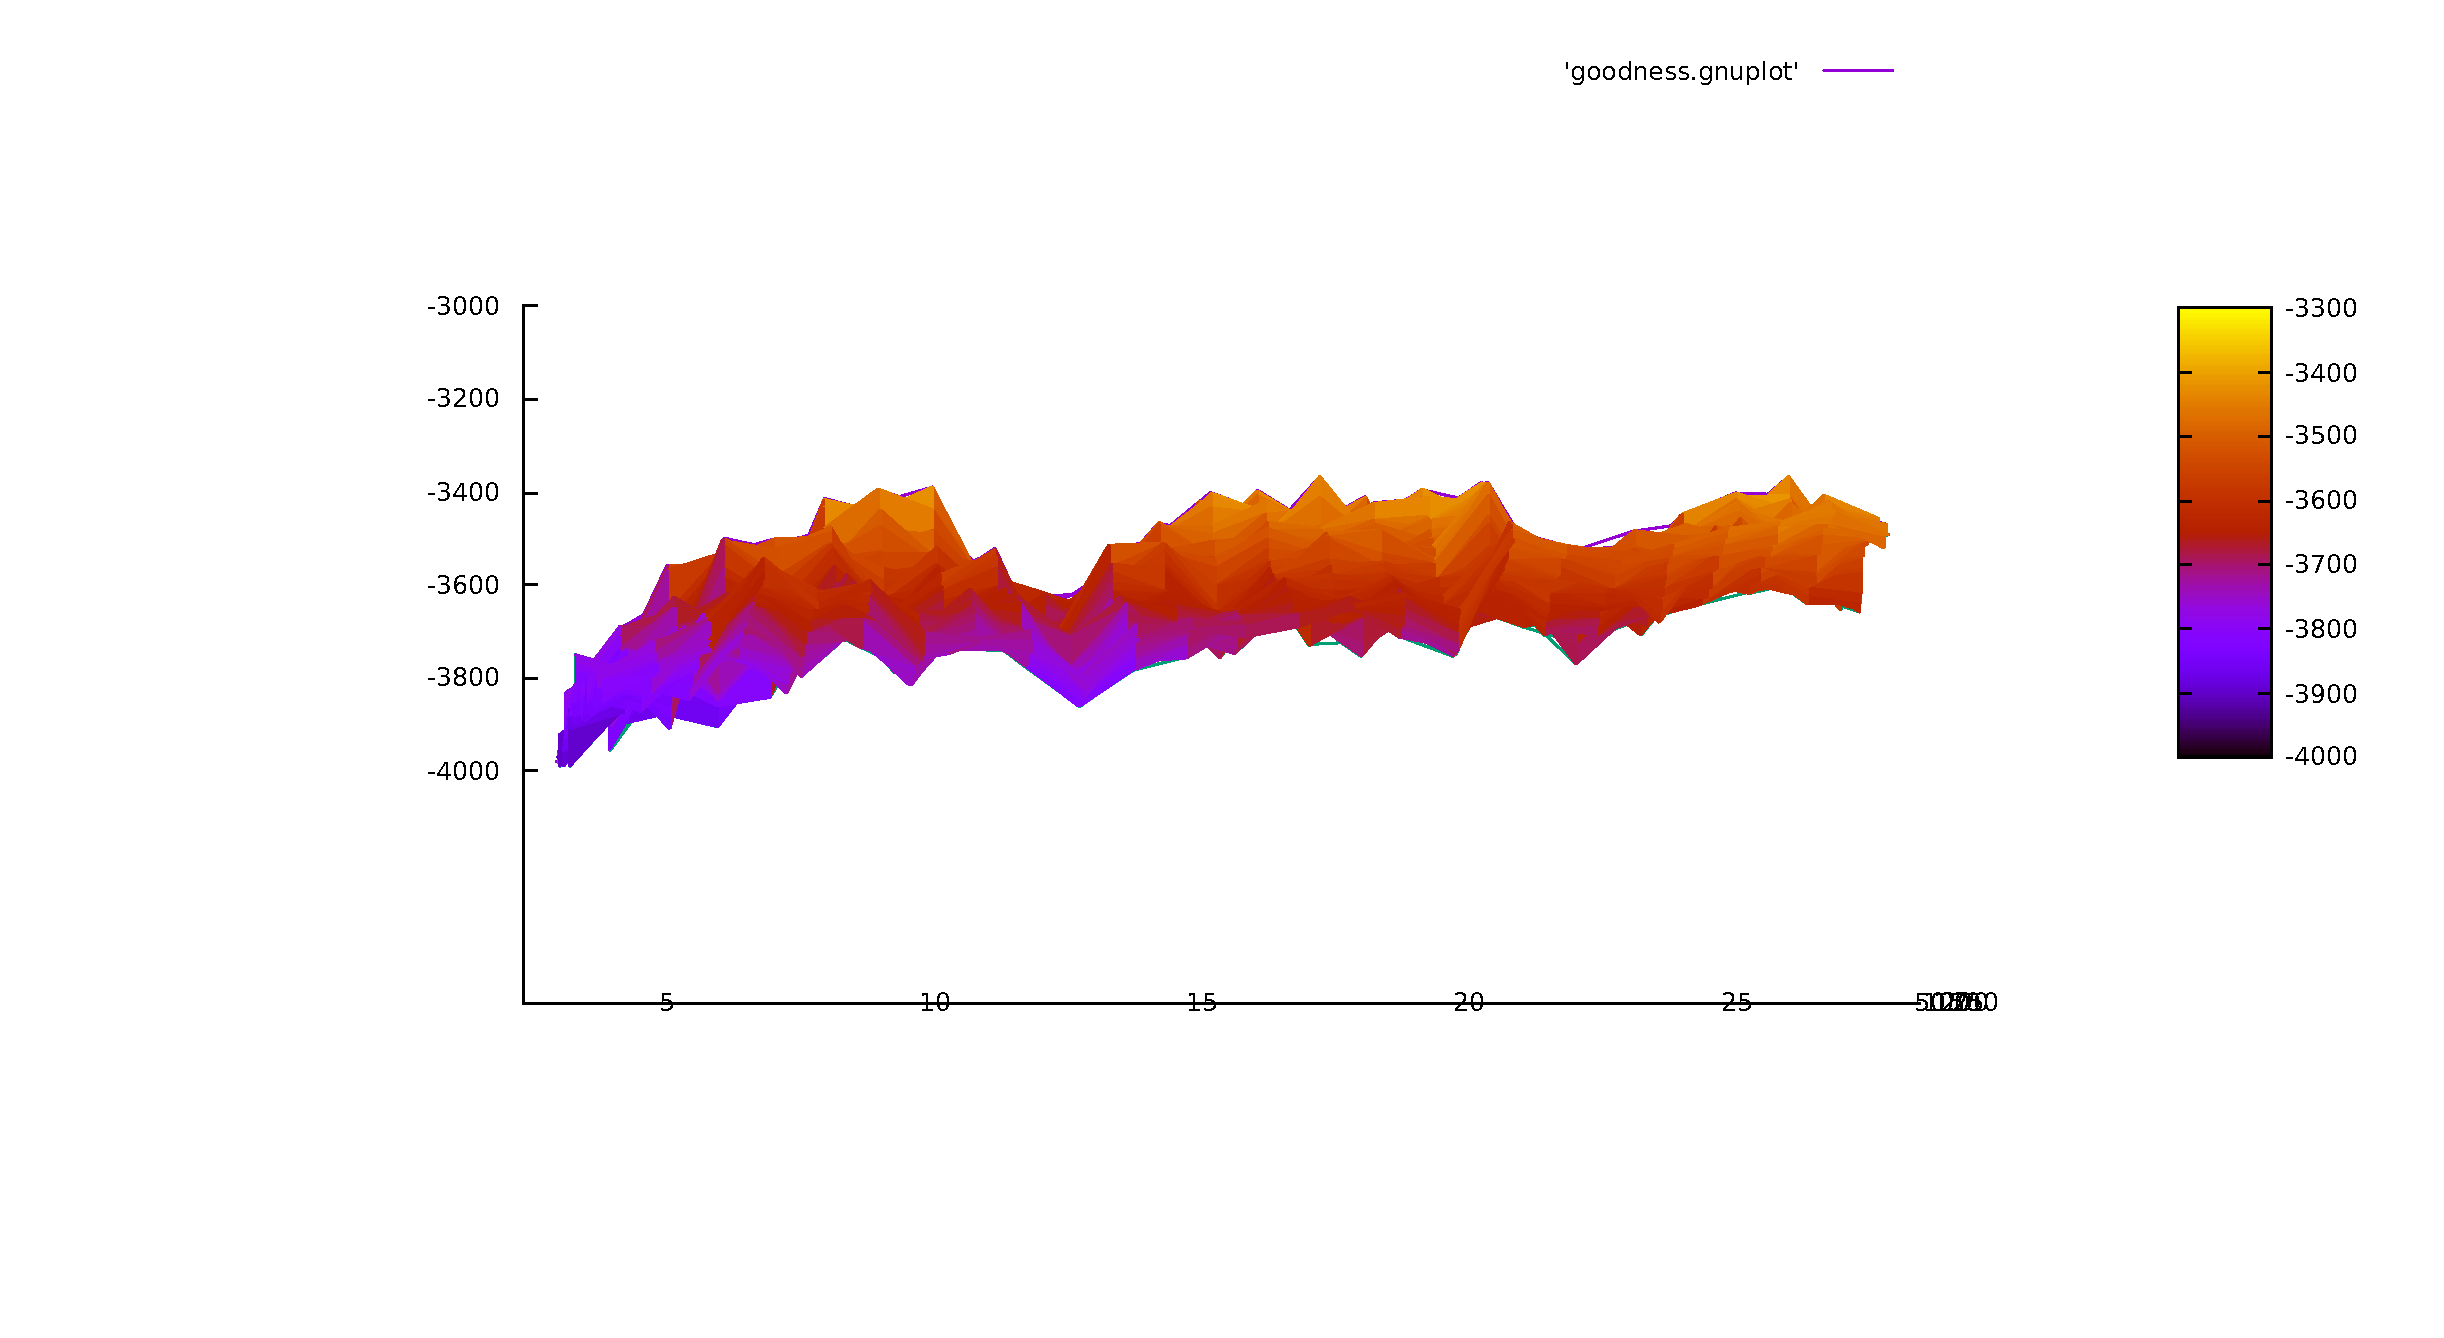
\includegraphics[scale=0.4]{k.pdf}
\caption{Bontà in funzione di $k$ e $h$, con $k$ in ascissa}
\end{figure}

\begin{figure}
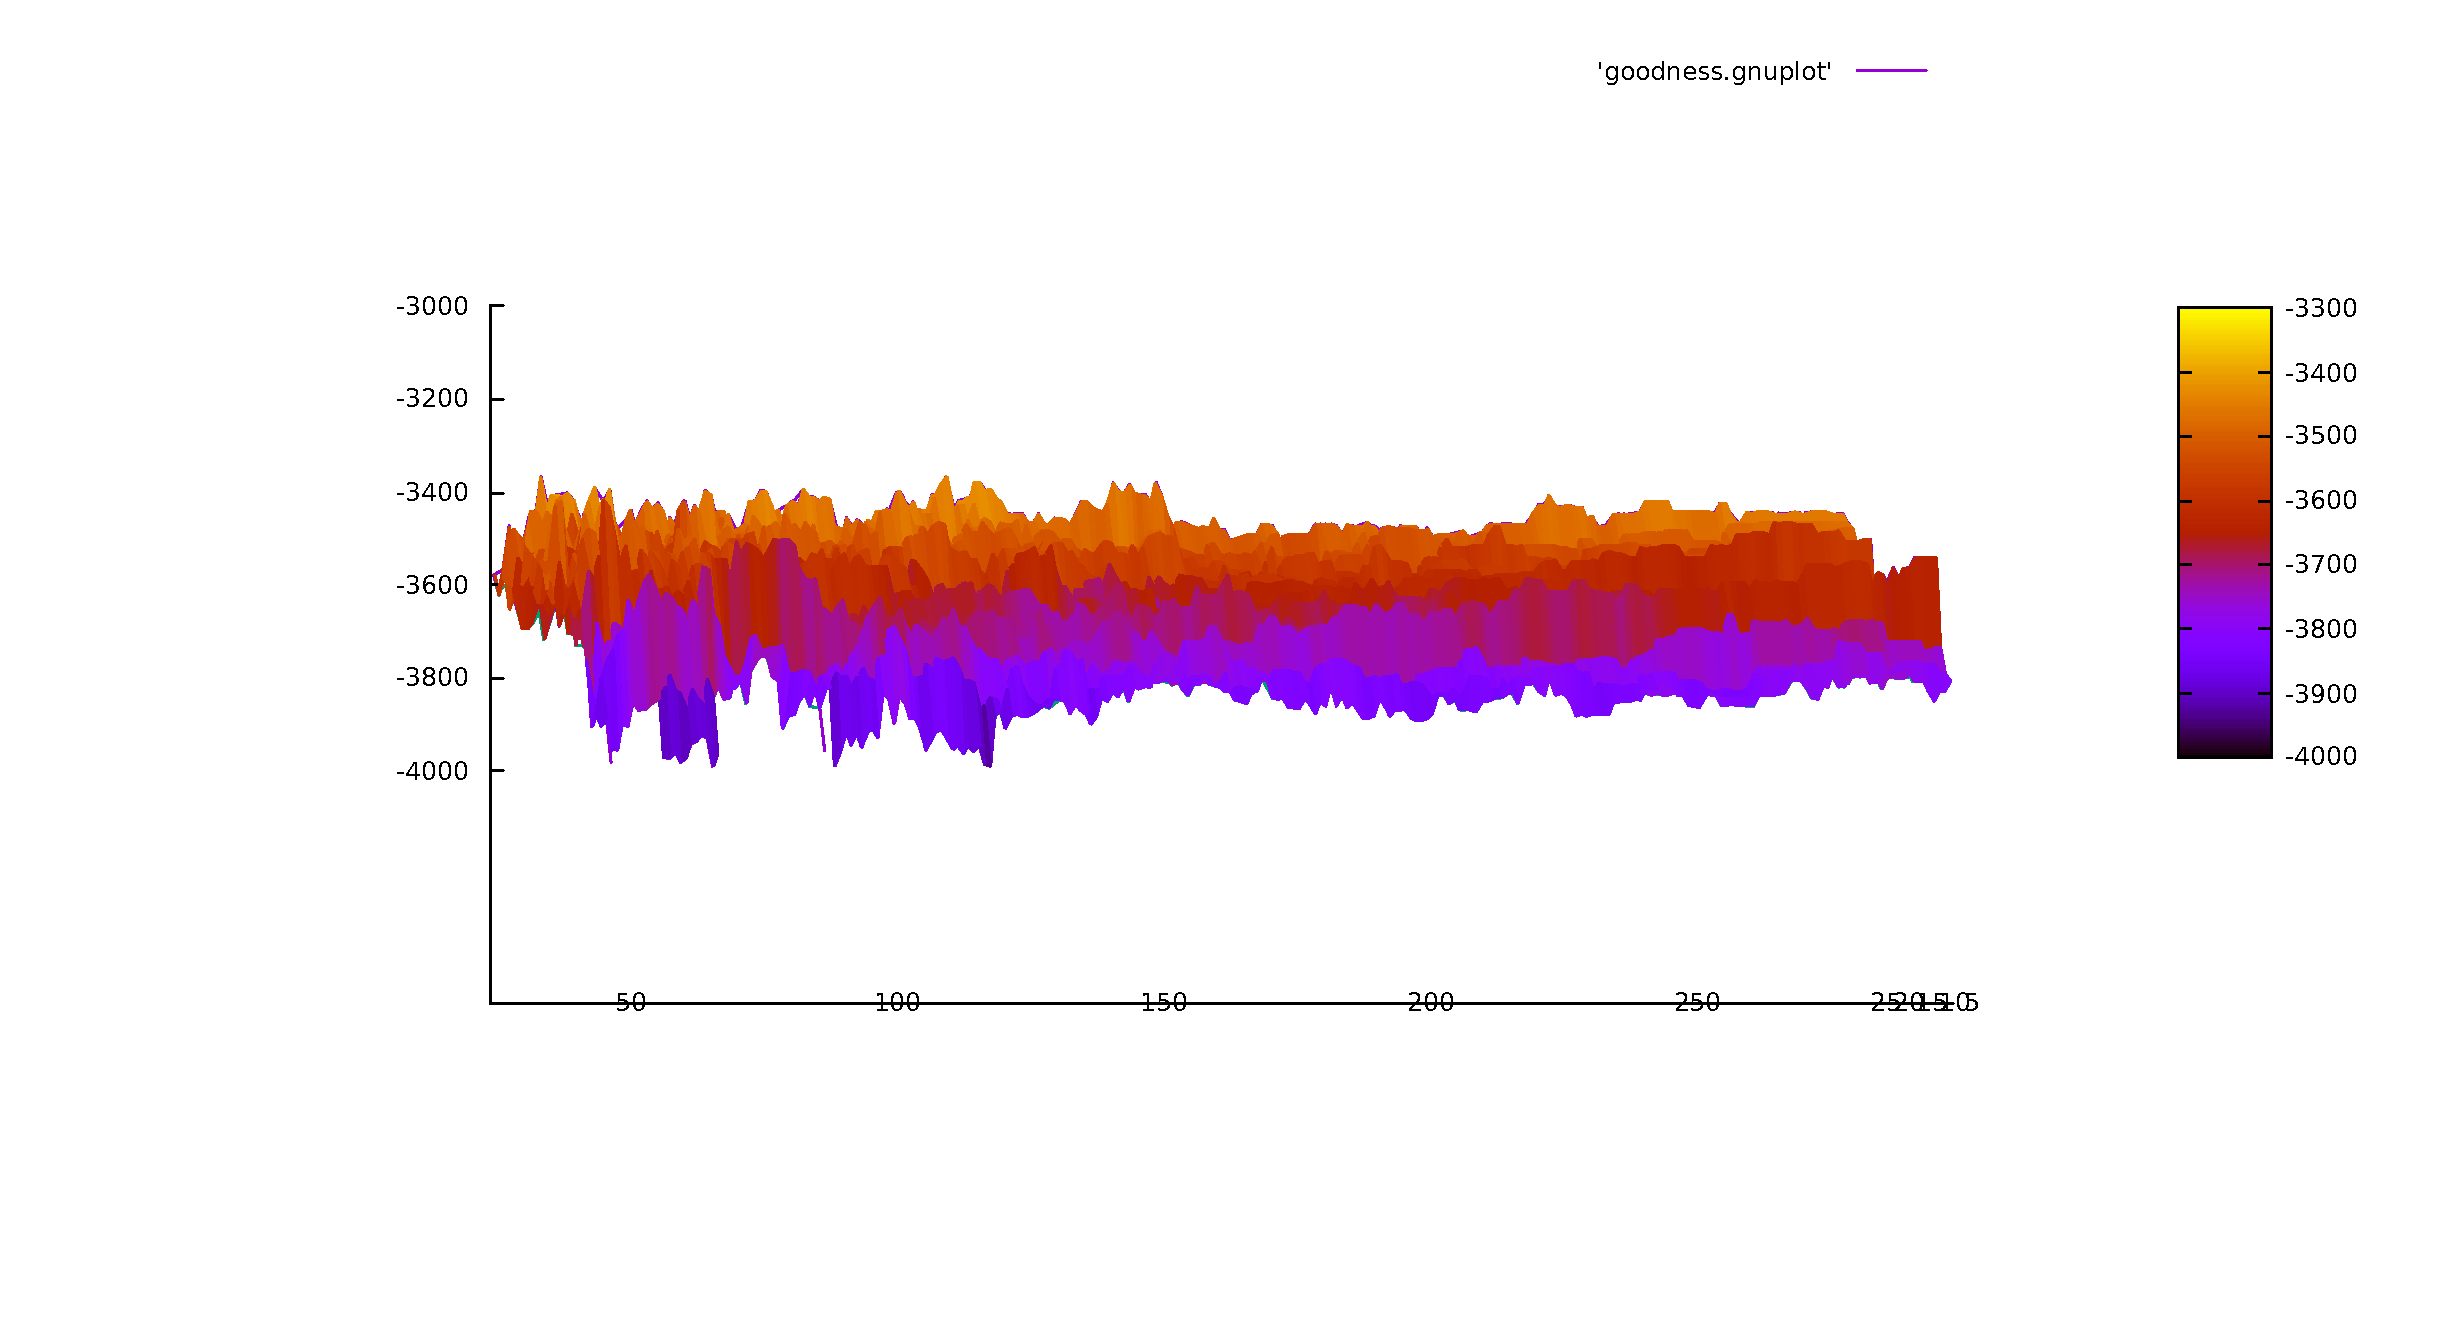
\includegraphics[scale=0.4]{h.pdf}
\caption{Bontà in funzione di $k$ e $h$, con $h$ in ascissa}
\end{figure}

\begin{figure}
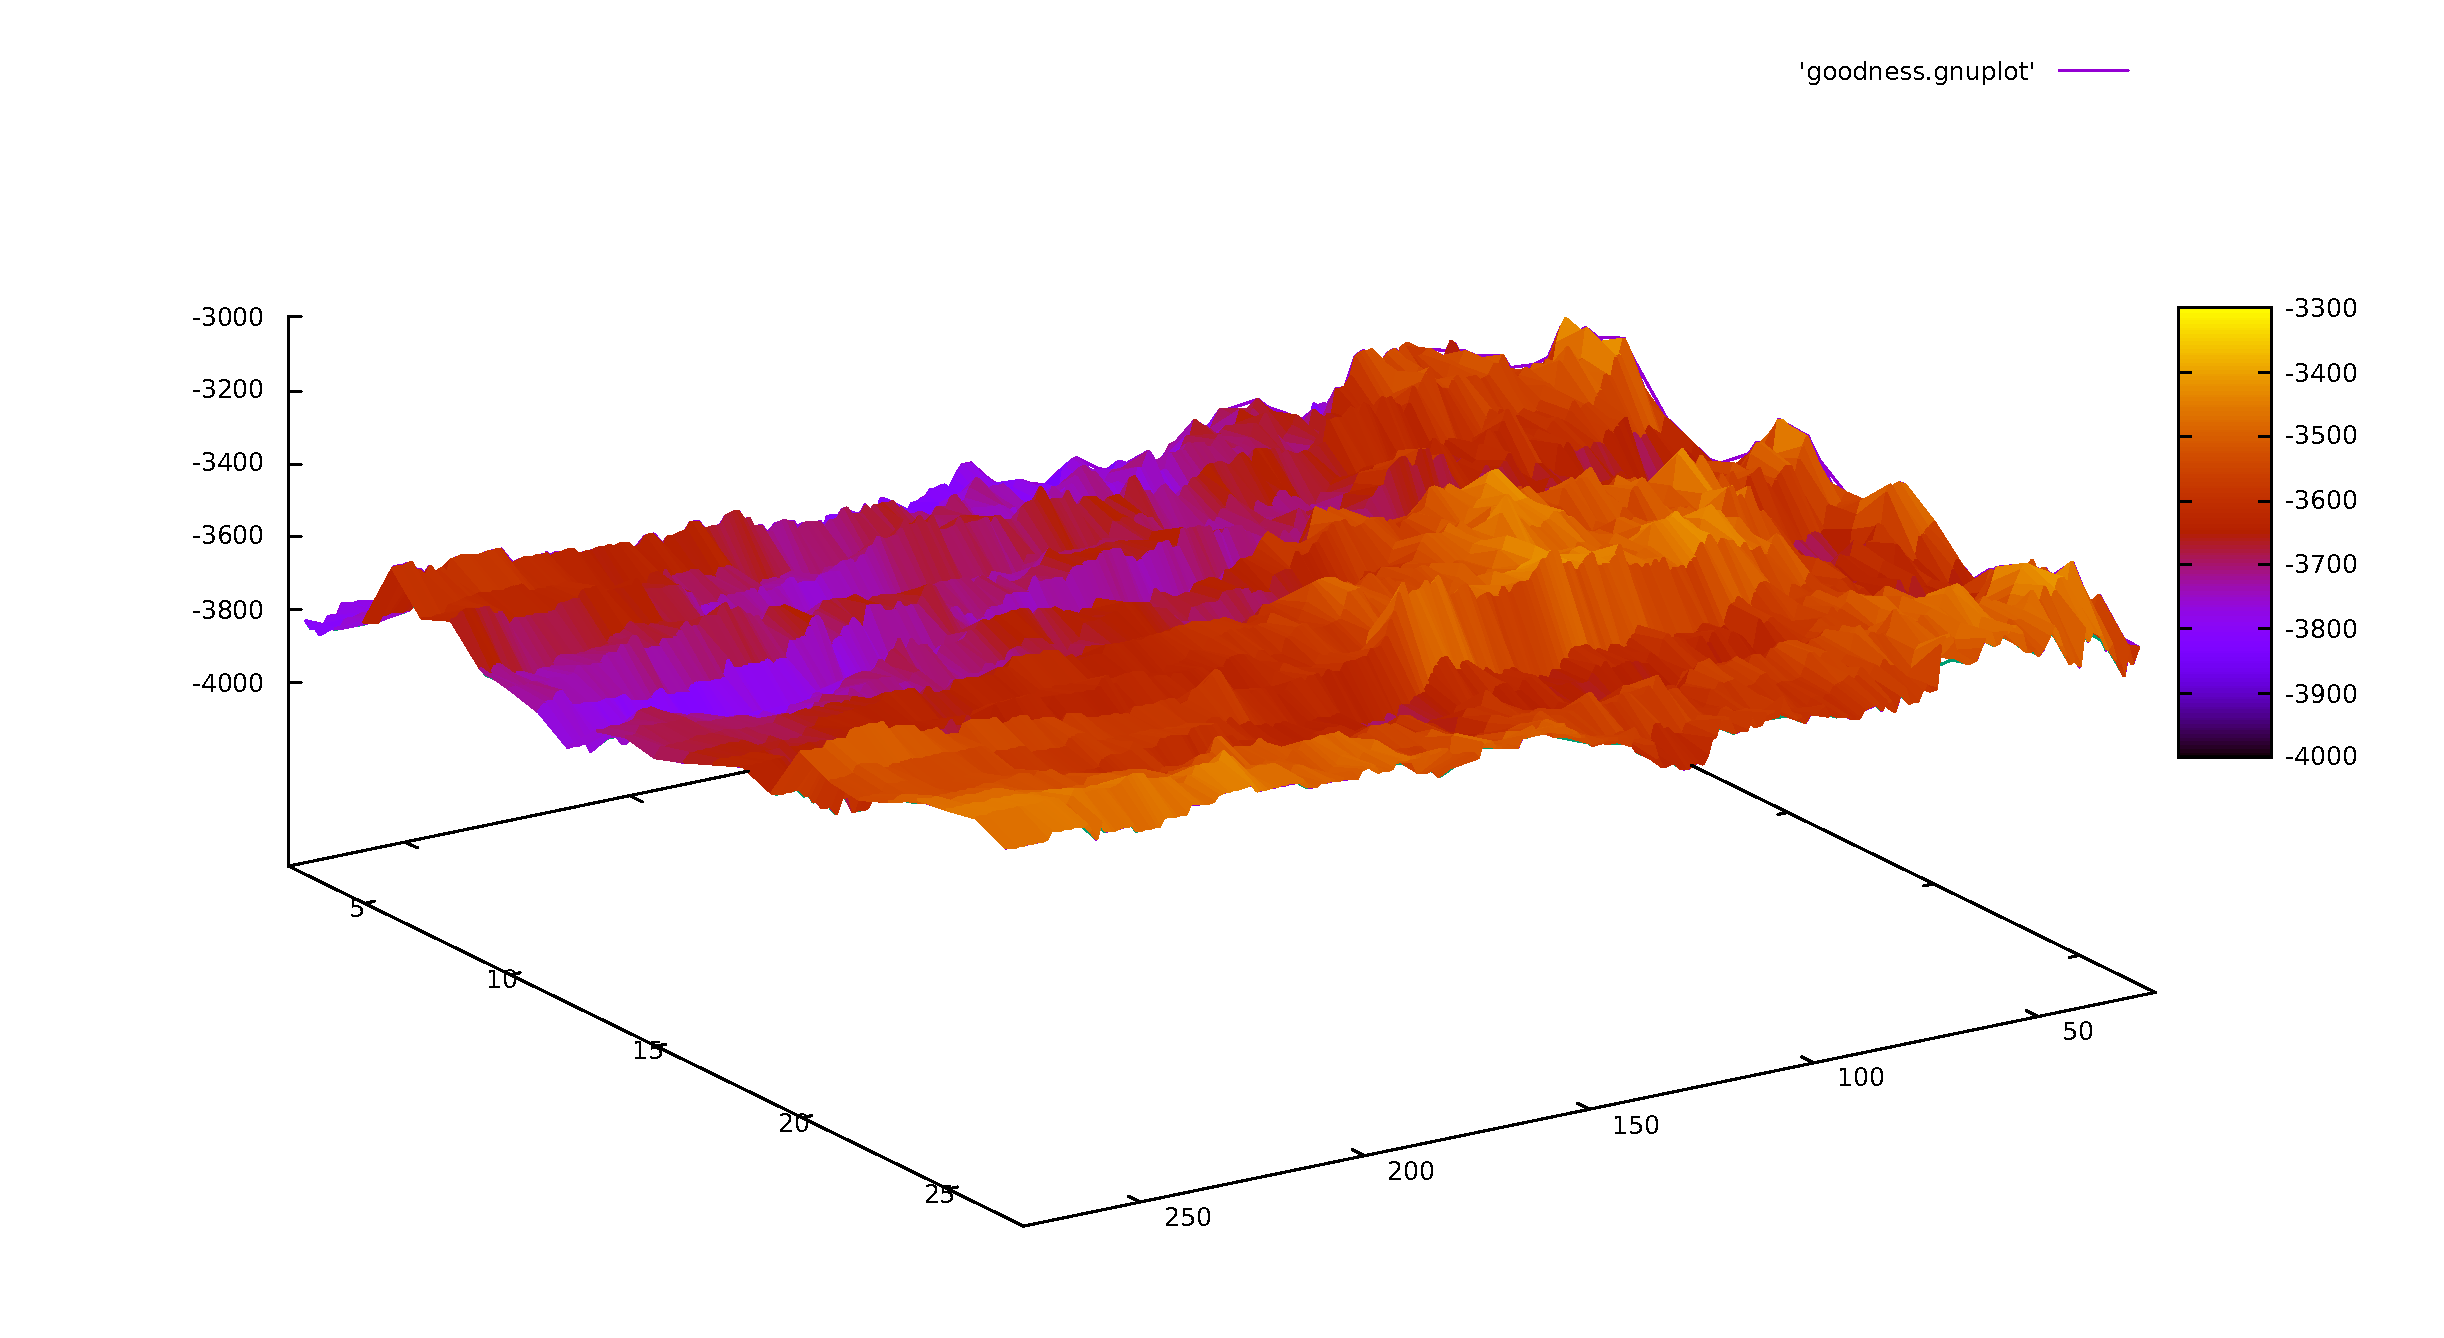
\includegraphics[scale=0.4]{3.pdf}
\caption{Bontà in funzione di $k$ e $h$}
\end{figure}

\end{document}
